\documentclass[../main.tex]{subfiles}

\begin{document}

\begin{definition}
A $n$-\textbf{simplex}\index{Simplex} $\Delta^n$ is the convex hull of $n+1$ general positioned points $v_0,\cdots,v_{n+1}$, called its \textbf{vertices}\index{Vertex}, a \textbf{face}\index{Face} is the convex hull of some vertices
\end{definition}

\begin{definition}\label{Scissors conguence}
A \textbf{polytope}\index{Polyhedron} $P$ is such that $P=\Delta_1\cup\cdots\cup \Delta_m$, where $\Delta_i$'s are simplices and the interiors of $\Delta_i$ are disjoint, and $\Delta_i\cap\Delta_j$ is precisely a common face \par
We say $P$ is a \textbf{generalized polytope}\index{Generalized polytope} if without the last condition
\begin{center}
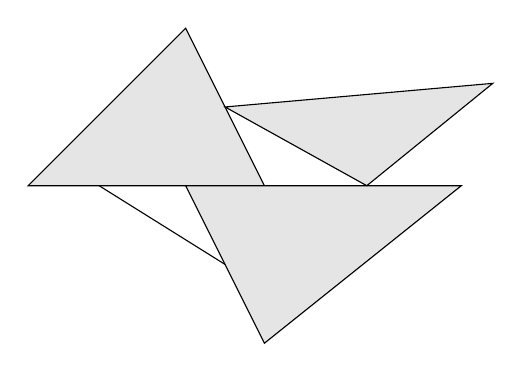
\begin{tikzpicture}
\coordinate (a) at (-1,2);
\coordinate (b) at (-3,0);
\coordinate (c) at (0,0);
\coordinate (d) at (-1,0);
\coordinate (e) at (0,-2);
\coordinate (f) at (2.5,0);
\coordinate (g) at (-0.5,1);
\coordinate (h) at (1.3,0);
\coordinate (i) at (2.9,1.3);
\coordinate (j) at (-2.1,0);
\coordinate (k) at (-0.5,-1);
\filldraw[fill=gray!20!white,draw=black](a)--(b)--(c)--cycle;
\filldraw[fill=gray!20!white,draw=black](d)--(e)--(f)--cycle;
\filldraw[fill=gray!20!white,draw=black](g)--(h)--(i)--cycle;
\draw(j)--(k);
\end{tikzpicture}
\end{center}
Suppose $P_1,P_2$ are polyhedra, we write $P=P_1\sqcup P_2$ if $P=P_1\cup P_2$ and the interiors of $P_1,P_2$ are disjoint. Therefore, any polyhedron $P$ must have a finite decomposition into polyhedra $P=P_1\sqcup\cdots\sqcup P_m$ \par
we say $P$ is \textbf{scissors congruent}\index{scissors congruent}(s.c.) to $Q$, denote $P\sim Q$, if there are decompositions $P=P_1\sqcup\cdots\sqcup P_m$, $Q=Q_1\sqcup\cdots\sqcup Q_m$ such that $Q_i=g_iP_i$, where $g_i\in \mathrm{Isom}(\mathbb R^n)$ is an isometry, we can also define more generally $G$-scissors congruence $\underset{G}{\sim}$, meaning $g_i\in G\leq \mathrm{Isom}(\mathbb R^n)$
\end{definition}

\begin{remark}
Two dimensional polytopes are called \textbf{polygons}\index{Polygon}, and three dimensional polytopes are called \textbf{polyhedrons}\index{Polyhedron}
\end{remark}

\begin{example}

\end{example}

\begin{theorem}\label{P,Q s.c. <=> P,Q have same area}
Suppose $P,Q$ are polygons in $\mathbb R^2$, $P\sim Q$ iff $\mathrm{Area}(P)=\mathrm{Area}(Q)$
\end{theorem}

\begin{proof} $\\$
\textbf{Step I: } Each polygon is triangulizable
\begin{center}
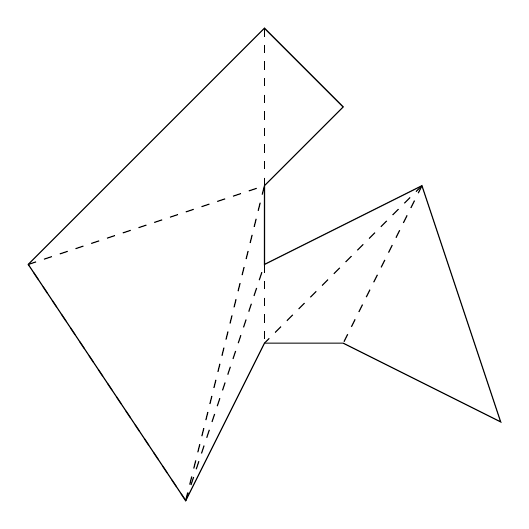
\begin{tikzpicture}
\coordinate (a) at (0,0);
\coordinate (b) at (-2,3);
\coordinate (c) at (1,6);
\coordinate (d) at (2,5);
\coordinate (e) at (1,4);
\coordinate (f) at (1,3);
\coordinate (g) at (3,4);
\coordinate (h) at (4,1);
\coordinate (i) at (2,2);
\coordinate (j) at (1,2);
\draw(a)--(b)--(c)--(d)--(e)--(f)--(g)--(h)--(i)--(j)--cycle;
\draw[dashed](a)--(b);
\draw[dashed](a)--(e);
\draw[dashed](a)--(f);
\draw[dashed](b)--(e);
\draw[dashed](c)--(e);
\draw[dashed](f)--(j);
\draw[dashed](g)--(i);
\draw[dashed](g)--(j);
\end{tikzpicture}
\end{center}
\textbf{Step II: } Each triangle is scissors congruent to a rectangle
\begin{center}
\begin{tikzpicture}
\draw(-1,0)--(0,2)--(3,0)--cycle;
\draw[dashed](-0.5,1)--(1.5,1);
\draw[dashed](0,1)--(0,2);

\draw[xshift=4.5cm,->](-1,0.5)--(1,0.5);

\begin{scope}[xshift=7cm]
\draw(-1,0)--(-1,1)--(3,1)--(3,0)--cycle;
\draw[dashed](-1,0)--(-0.5,1);
\draw[dashed](1.5,1)--(3,0);
\end{scope}
\end{tikzpicture}
\end{center}
\textbf{Step III: }A rectangle with the shorter side between $\dfrac{1}{2}$ and $1$

\textbf{Step IV: }
\begin{center}
\begin{tikzpicture}
\draw(0,0)--(4,0)--(4,0.75)--(0,0.75)--cycle;
\begin{scope}
\clip(0,0) rectangle (4,0.75);
\path[name path=line 1](3,0)--(3,3);
\path[name path=line 2](0,1)--(4,0);
\path[name intersections={of= line 1 and line 2, by=x}];
\draw[dashed](3,0)--(x);
\draw[dashed](0,1)--(4,0);
\end{scope}
\draw[xshift=5.5cm,->](-1,0.5)--(1,0.5);
\begin{scope}[xshift=7cm]
\draw(0,0)--(3,0)--(3,1)--(0,1)--cycle;
\begin{scope}
\clip(0,0) rectangle (3,1);
\path[name path=line 1](0,0.75)--(3,0.75);
\path[name path=line 2](0,1)--(4,0);
\path[name intersections={of= line 1 and line 2, by=x}];
\draw[dashed](0,0.75)--(x);
\draw[dashed](0,1)--(4,0);
\end{scope}
\end{scope}
\end{tikzpicture}
\end{center}
\end{proof}

\begin{trivlist}
\item[\hskip \labelsep  \textbf{Hilbert's third problem.}]
Is there any two polyhedra of the same volume which is not scissors congruent
\end{trivlist}
% This way you can change your title into anything you want
\begin{trivlist}
\item[\hskip \labelsep  \textbf{Answer.}]
YES!
\end{trivlist}

\begin{definition}
Given a polyhedron $P$, we can define \textbf{Dehn invariant}\index{Dehn invariant}
\[D(P)=\sum_{e}l(e)\otimes\dfrac{\theta(e)}{\pi}\in\mathbb R\underset{\mathbb Z}{\otimes}\mathbb R/\mathbb Z\]
Where $e$ runs over all the edges of $P$, $l(e)$ is the length of $e$, $\theta(e)$ is the dehedral angle
\end{definition}

\begin{theorem}\label{Dehn invariant is invariant of s.c.}
$D$ is an invariant of scissors congruence
\end{theorem}

\begin{proof}

\end{proof}

\begin{lemma}\label{a tensor b is not zero in R tensor R mod Z if b is irrational}
If $b\notin\mathbb Q$, then $a\otimes b\in\mathbb R\underset{\mathbb Z}{\otimes}\mathbb R/\mathbb Z$ is not zero
\end{lemma}

\begin{proof}
We can define a $\mathbb Z$-bilinear map $\langle a\rangle\times\langle b\rangle\to\mathbb R/\mathbb Z,$ $(na,mb)\mapsto(nmb)$, which induces a homomorphism $\langle a\otimes b\rangle=\langle a\rangle\otimes\langle b\rangle\to\mathbb R/\mathbb Z,$ $nm(a\otimes b)=na\otimes mb\mapsto(nmb)$, this is not a zero map, thus $a\otimes b$ is not zero
\end{proof}

\begin{example}
The Dehn invariant of a cube of side length $l$ is
\[6l\otimes\dfrac{1}{2}=0\]
The Dehn invariant of a tetrahedron of side length $l$ is
\[4l\otimes\dfrac{\theta}{\pi}\]
Where $\cos\theta=\dfrac{1}{3}$ \par
Let's show that $\dfrac{\theta}{\pi}\notin\mathbb Q$, suppose otherwise, then there is a positive integer $k$ such that $\cos k\theta=0$, let's show $\cos k\theta=\dfrac{a_k}{3^k}$, $3\nmid a_k$ by induction, when $k=1$, $\cos\theta=\dfrac{1}{3},3\nmid1$
\begin{align*}
\cos(k+1)\theta&=2\cos k\theta\cos\theta-\cos(k-1)\theta \\
&=2\dfrac{a_k}{3^k}\dfrac{1}{3}-\dfrac{a_{k-1}}{3^{k-1}} \\
&=\dfrac{2a_k-9a_{k-1}}{3^{k+1}}
\end{align*}
$3\mid9a_{k-1}$ but $3\nmid2a_k$ \par
According to Lemma \ref{a tensor b is not zero in R tensor R mod Z if b is irrational}, we know the Dehn invariant of a tetrahedron isn't zero, thus a cube and a tetrahedron can never be scissors congruent due to Theorem \ref{Dehn invariant is invariant of s.c.}
\end{example}

\begin{theorem}[Sydler]
Suppose $P,Q$ are polyhedra in $\mathbb R^3$, $P\sim Q$ iff $\mathrm{Volume}(P)=\mathrm{Volume}(Q)$ and $D(P)=D(Q)$
\end{theorem}

\begin{proof}

\end{proof}

\begin{definition}
Suppose $X$ is a metric space with the notion of a polytope, for example $\mathbb R^n$, $S^n$, $\mathbb H^n$ \par
The \textbf{scissors congruence group}\index{Scissors congruence group} $\mathcal P(X)$ is defined to the free abelian group generated by polytopes $[P]$, modulo relations: \par
\textbf{i: }$[P]=[P_1]+[P_2]$, for $P=P_1\sqcup P_2$ \par
\textbf{ii: }$[gP]=[P]$, for $g\in \mathrm{Isom}(\mathbb R^n)$ \par
$\mathrm{Isom}(\mathbb R^n)$ is the Isometry group of $\mathbb R^n$ \par
We can also define more generally $\mathcal P(X,G)$, meaning $g\in G\leq \mathrm{Isom}(\mathbb R^n)$ \par
$P$ and $Q$ is \textbf{stably scissors congruent}\index{Stable scissors congruence} if $P\sqcup R\sim Q\sqcup R'$
\end{definition}

\begin{proposition}
If $P,Q$ are scissors congruent, $[P]=[Q]$
\end{proposition}

\begin{proof}
By Definition \ref{Scissors conguence}, $P=P_1\sqcup\cdots\sqcup P_m$, $Q=Q_1\sqcup\cdots\sqcup Q_m$ and $Q_i=g_iP_i$, $g_i\in G$, thus $[P]=[P_1]+\cdots+[P_m]=[Q_1]+\cdots+[Q_m]=[Q]$
\end{proof}

\begin{remark}
We can give isometric classes of polytopes a commutative monoid stucture, then $\mathcal P(X)$ is the Grothendieck K-group, $[P]=[Q]$ iff $P\sqcup R\sim Q\sqcup R'$, where $R'=gR$
\end{remark}

\begin{lemma}\label{Lemma for Zylev's theorem}
Suppose $P,Q$ are generalized polytopes, and $\mathrm{Volume}(P)>\mathrm{Volume}(Q)$, then there exists a generalized polytope $R\subseteq P$ such that $Q\sim R$
\end{lemma}

\begin{proof}
Consider dividing into small cubes \par
On $S^2$, we can consider barycentric subdivision of the tetrahedron over and over again
\end{proof}

\begin{theorem}[Zylev]\label{Zylev's theorem}
Suppose $G$ acts on $X$ transitively, stable scissors congruence implies scissors congruence
\end{theorem}

\begin{proof}
Let's only consider the special case $X=\mathbb R^n$, $G=\mathrm{Isom(\mathbb R^n)}$, if $[P]=[Q]$, then $P\sqcup R\sim Q\sqcup R'$, where $R'=gR$, it suffices to prove: if $Y=P\bigcup\bigcup_{i=1}^kP_i=Q\bigcup\bigcup_{i=1}^kQ_i$ and $P_i\sim Q_i$, then $P\sim Q$, we also assume that $\mathrm{Volume}(Y)>3\mathrm{Volume}(P_i)$, by then Lemma \ref{Lemma for Zylev's theorem} there exists a generalized polytope $T_k\subseteq Y-P_k\cup Q_k$ such that $T_k\sim P_k\cap Q_k$, schematically shown as follow
\begin{center}
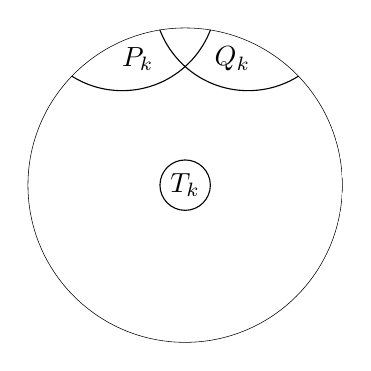
\begin{tikzpicture}[scale=0.4]
\clip (0,0) circle (5);
\draw (0,0) circle (5);
\draw (0,0) circle (0.8);
\draw (-2,6) circle (3);
\draw (2,6) circle (3);
\node at (-1.5,4) {$P_k$};
\node at (1.5,4) {$Q_k$};
\node at (0,0) {$T_k$};
\end{tikzpicture}
\end{center}
Then we would have
\begin{center}
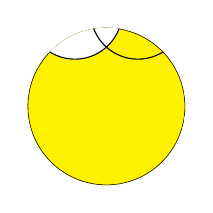
\begin{tikzpicture}[scale=0.2]
\clip (0,0) circle (5);
\filldraw[yellow] (0,0) circle (5);
\draw (0,0) circle (5);
\filldraw[white] (-2,6) circle (3);
\draw (-2,6) circle (3);
\draw (2,6) circle (3);
\end{tikzpicture}
\begin{tikzpicture}[scale=0.2]
\node at (0,-4) {$\,$};
\node at (0,0) {$\sim$};
\end{tikzpicture}
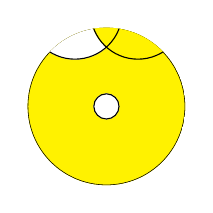
\begin{tikzpicture}[scale=0.2]
\clip (0,0) circle (5);
\filldraw[yellow] (0,0) circle (5);
\draw (0,0) circle (5);
\filldraw[white] (0,0) circle (0.8);
\draw (0,0) circle (0.8);
\filldraw[white] (-2,6) circle (3);
\filldraw[yellow] (2,6) circle (3);
\draw (-2,6) circle (3);
\draw (2,6) circle (3);
\end{tikzpicture}
\begin{tikzpicture}[scale=0.2]
\node at (0,-4) {$\,$};
\node at (0,0) {$\sim$};
\end{tikzpicture}
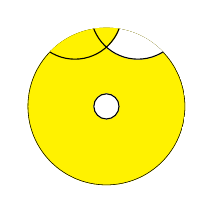
\begin{tikzpicture}[scale=0.2]
\clip (0,0) circle (5);
\filldraw[yellow] (0,0) circle (5);
\draw (0,0) circle (5);
\filldraw[white] (0,0) circle (0.8);
\draw (0,0) circle (0.8);
\filldraw[white] (2,6) circle (3);
\filldraw[yellow] (-2,6) circle (3);
\draw (2,6) circle (3);
\draw (-2,6) circle (3);
\end{tikzpicture}
\begin{tikzpicture}[scale=0.2]
\node at (0,-4) {$\,$};
\node at (0,0) {$\sim$};
\end{tikzpicture}
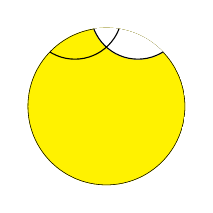
\begin{tikzpicture}[scale=0.2]
\clip (0,0) circle (5);
\filldraw[yellow] (0,0) circle (5);
\draw (0,0) circle (5);
\filldraw[white] (2,6) circle (3);
\draw (2,6) circle (3);
\draw (-2,6) circle (3);
\end{tikzpicture}
\end{center}
Thus $P\bigcup\bigcup_{i=1}^{k-1}P_i\sim Q\bigcup\bigcup_{i=1}^{k-1}Q_i$, by induction, we get $P\sim Q$
\end{proof}

\end{document}